\section{Color Shift Keying}
\label{sec:csk}
\graphicspath{{_MIMOColor/figures_csk/}}

\subsection{Linear System Model}
\label{subsec:cskLinear}
The linear CSK model treats the CIE-CS as a linear space to analyze CSK performance. This implies the inherent assumption that when irradiance from multiple transmitting elements is combined, the chromaticity coordinates of the resulting SPD is a linear combination of the chromaticity coordinates of the SPDs of individual transmitting elements. If P$_{n}$; $n\in$ \{i, j, k\} is the normalized radiant flux at the transmit or receive device associated with band $n$, Eq.(\ref{eqLIN}) below taken from the standard provides the implied mathematical relationships between chromaticity coordinates of all bands and that of resultant SPD.

\begin{equation}
	\begin{aligned}
	x_{\text{p}} &= \text{P}_{\text{i}}x_{\text{i}} + \text{P}_{\text{j}}x_{\text{j}} + \text{P}_{\text{k}}x_{\text{k}}\\
	y_{\text{p}} &= \text{P}_{\text{i}}y_{\text{i}} + \text{P}_{\text{j}}y_{\text{j}} + \text{P}_{\text{k}}y_{\text{k}}\\
	1 &= \text{P}_{\text{i}} + \text{P}_{\text{j}} + \text{P}_{\text{k}}
\end{aligned}
\label{eqLIN}
\end{equation}

\afterpage{%
\clearpage
\begin{landscape}% Landscape page
\begin{figure}
	\centering
		%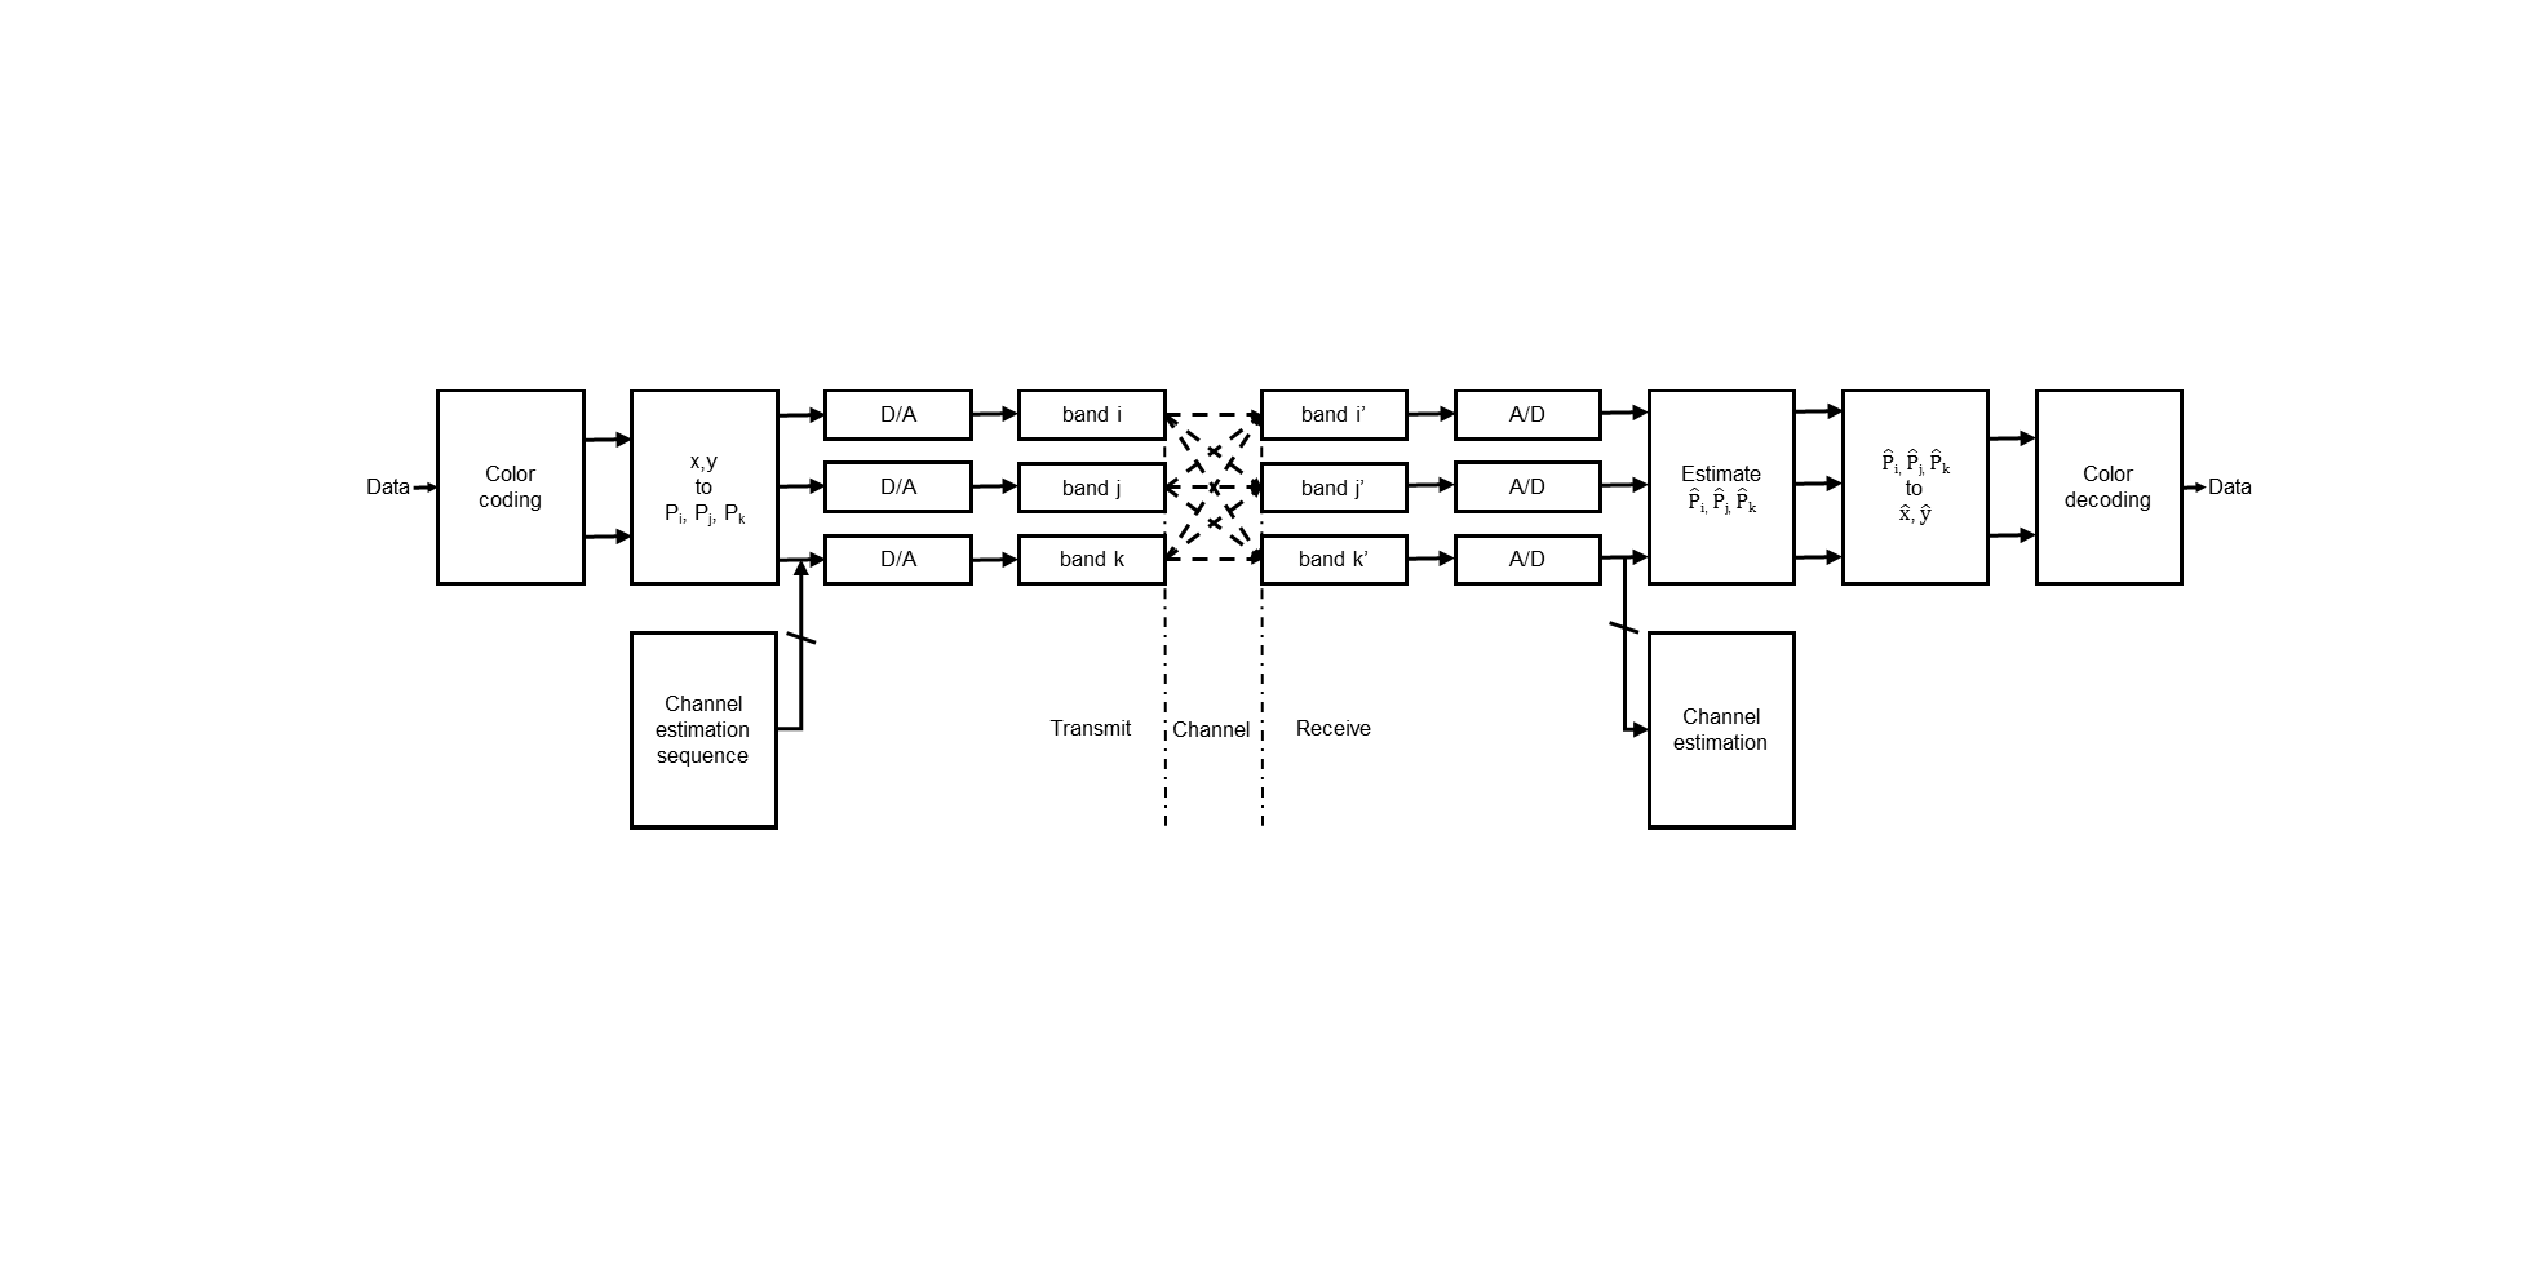
\includegraphics[trim={2.34in 2.78in 1.76in 2.47in}, clip=true, width=5.25in]{CSKBlockDiagram_1.eps}
		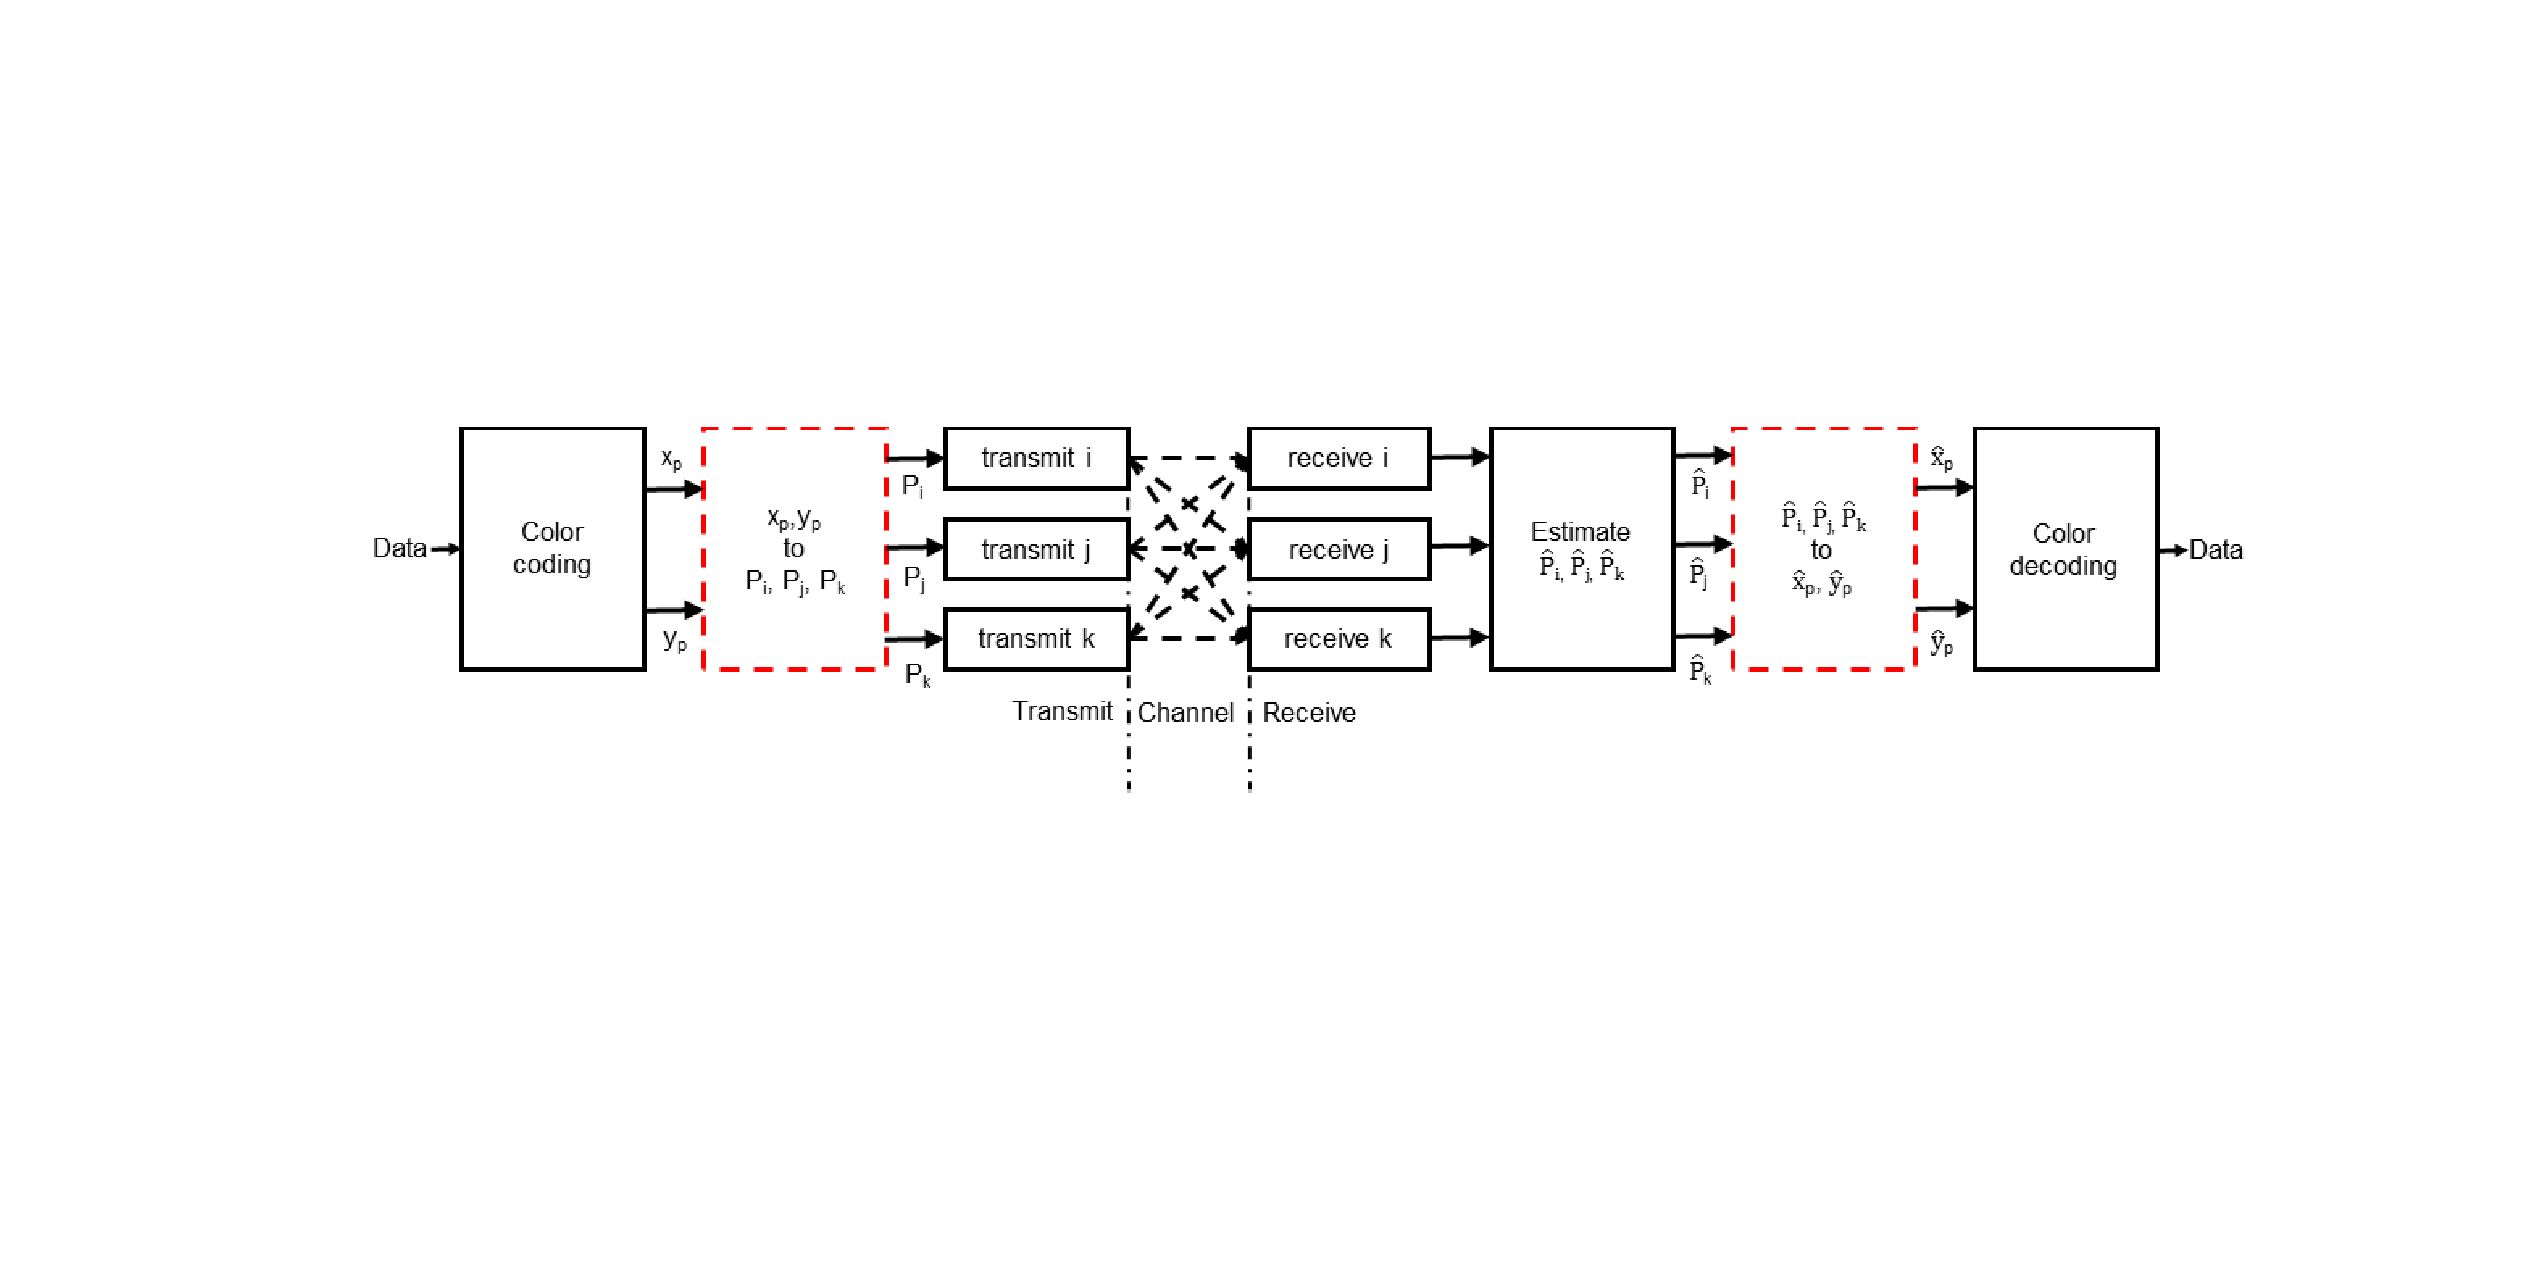
\includegraphics[trim={2.34in 2.78in 1.76in 2.47in}, clip=true, width=7.5in]{CSKBlockDiagram.eps}
	\caption{Block diagram of CSK signal chain. Implementation of red dashed blocks differentiates the linear and the non-linear system models.}
	\label{figCSKBD}
\end{figure}
\end{landscape}
\clearpage% Flush page
}

A block diagram of the CSK signaling chain is shown in \figurename{ }\ref{figCSKBD}. At the transmitting element, the data bit-stream is encoded to chromaticity coordinates ($x_{\text{p}}$, $y_{\text{p}}$) as computed from Table \ref{tMCSK}. Using Eq.(\ref{eqLIN}), normalized P$_{n}$ values are computed which are then scaled to achieve a given illumination target and thus transmit irradiance. A vector of scaled P$_{n}$ values then forms the transmit vector \vm{X}. Without loss of generality, unity electrical to optical conversion at transmitter and unity responsivity (optical to electrical conversion) at the receiver is assumed. Receiving element for band $n$ senses the incident flux and generates an electrical signal proportional to it. AWGN as computed from Eq.\eqref{eqNOISE} is then added to each band $n$ in the form of vector \vm{W}. The receiver output in presence of noise is represented by \vm{Y}. With the knowledge of the channel state and the receiver output, a least squares estimate of transmit vector $\hat{\vm{X}}$ is made using Eq.\eqref{eqXHAT}. Each element of $\hat{\vm{X}}$ then provides the estimates of transmitted flux represented by $\hat{\text{P}}_{n}$. Using these values, ($\hat{x}_{\text{p}}, \hat{y}_{\text{p}}$) are estimated using Eq.\eqref{eqLIN}. Nearest neighbor decoder then estimates the transmitted coordinate and recovers the transmitted information. Thus for the linear system model, Eq.\eqref{eqLIN} represents the ($x_{\text{p}}$, $y_{\text{p}}$) $\rightarrow  \text{P}_{n}$ and $\hat{\text{P}}_{n}\rightarrow$ ($\hat{x}_{\text{p}}$, $\hat{y}_{\text{p}}$) transformations for the red dashed blocks of \figurename{ }\ref{figCSKBD}.
%In this case the channel matrix \vm{H} is $n_{\text{rx}}\times n_{\text{tx}}$ dimensional identity matrix ($n_{\text{rx}}=n_{\text{tx}} = 3$).

Monte-carlo simulations are performed to compute performance of $M$-ary CSK under the linear model for all CBC$_{v}$ and \figurename{ }\ref{figBERvsSNR} shows the results. Performance of all CBCs is similar except CBC$_{7}$ and CBC$_{9}$ which perform slightly worse, but only by a margin of about 0.6 dB. This performance is as expected. As seen from Table \ref{tCBC}, CBC$_{7}$ is composed of CB$_{3}$, CB$_{2}$ and CB$_{0}$ whereas and CBC$_{9}$ is composed of CB$_{2}$, CB$_{1}$ and CB$_{0}$. Thus from values in Table \ref{tCB} and \figurename{ }\ref{figCBCcenters}, it can be seen that constellation points for other CBCs are the most spread out and have the large minimum distance between constellation points where as that for CBC$_{7}$ and CBC$_{9}$ have the shorter spread and have the smaller minimum distance between constellation points. SNR of at least 15 dB, 20 dB and 25 dB are needed to achieve a target minimum bit error rate (BER) of $10^{-3}$ under the linear model for $M$ = 4, 8 and 16 CSK respectively.

\afterpage{%
\clearpage
\begin{landscape}% Landscape page
\begin{figure}[t]
	\centering
		\begin{subfigure}{0.49\textwidth}
		\centering
			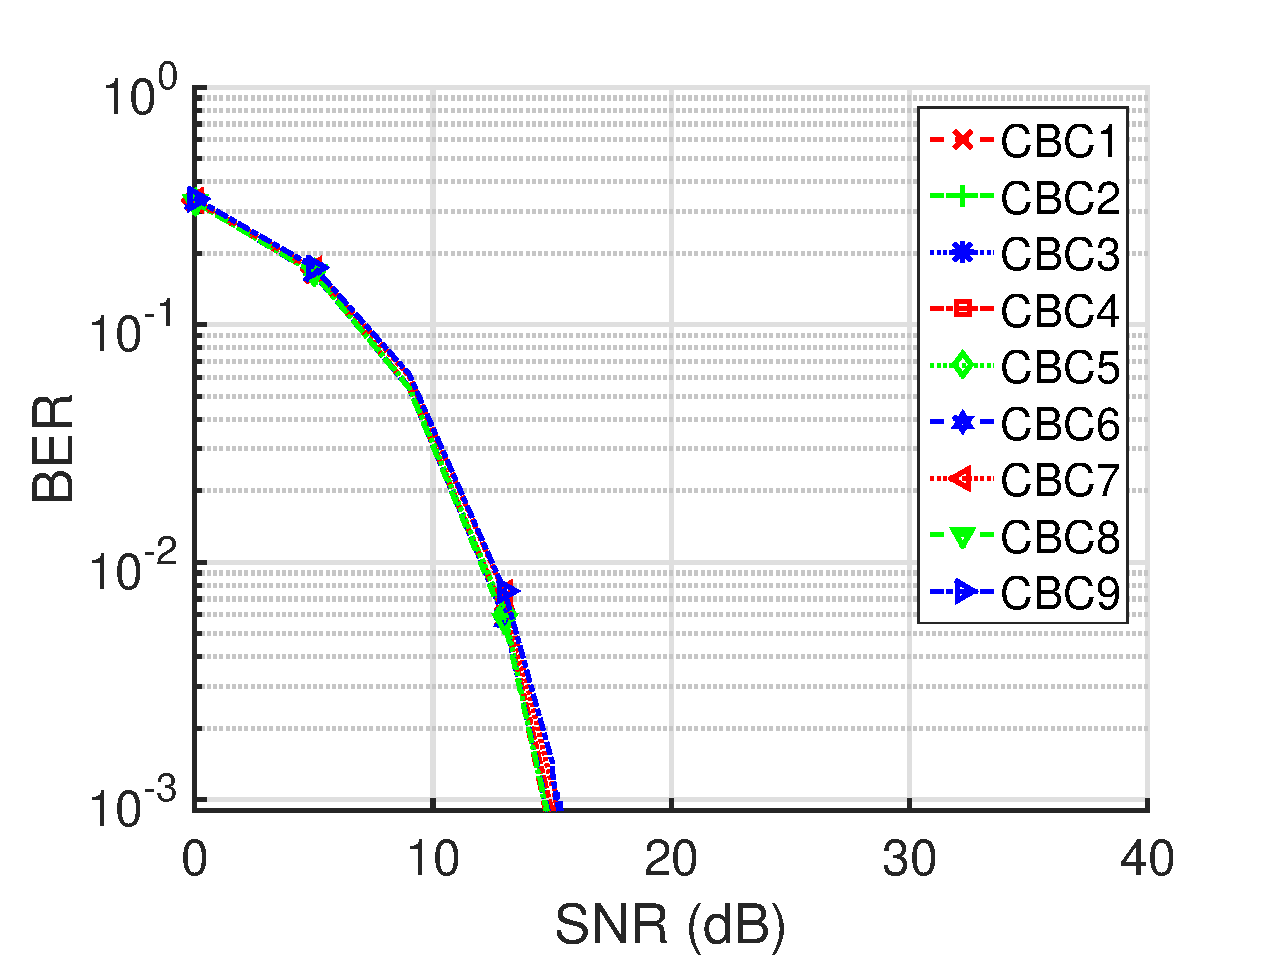
\includegraphics[trim={0.1in 0.0in 0.6in 0.3in}, clip=true, width=\textwidth]{M04_4-CSK_BERvsSNR.eps}
			\caption{4-CSK}
			\label{fig4SNR}
		\end{subfigure}
		%\hfill
		\begin{subfigure}{0.49\textwidth}
		\centering
			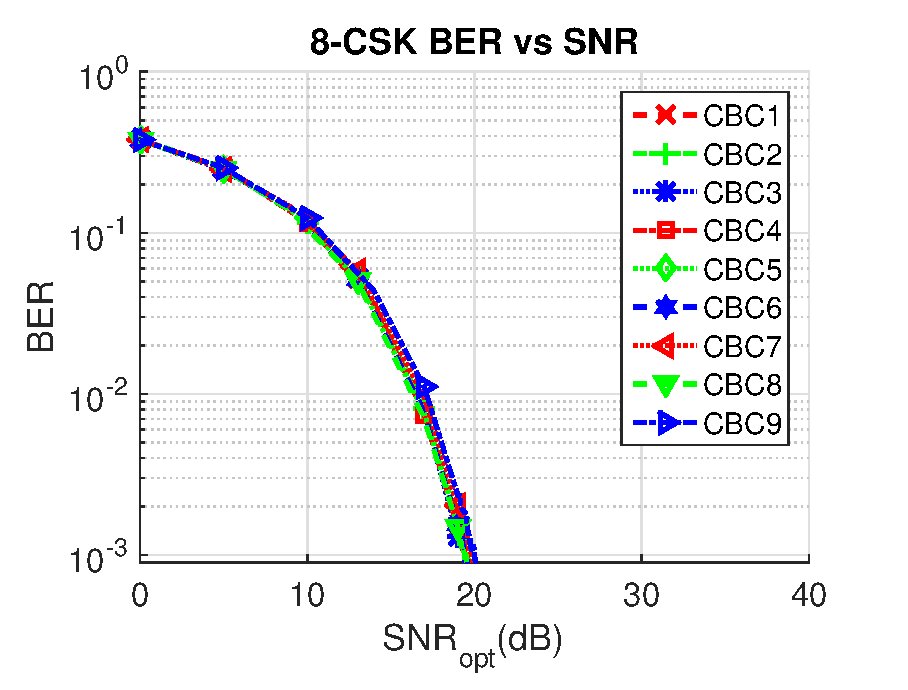
\includegraphics[trim={0.1in 0.0in 0.6in 0.3in}, clip=true, width=\textwidth]{M08_8-CSK_BERvsSNR.eps}
			\caption{8-CSK}
			\label{fig8SNR}
		\end{subfigure}
		%\vfill
		\begin{subfigure}{0.49\textwidth}
		\centering
			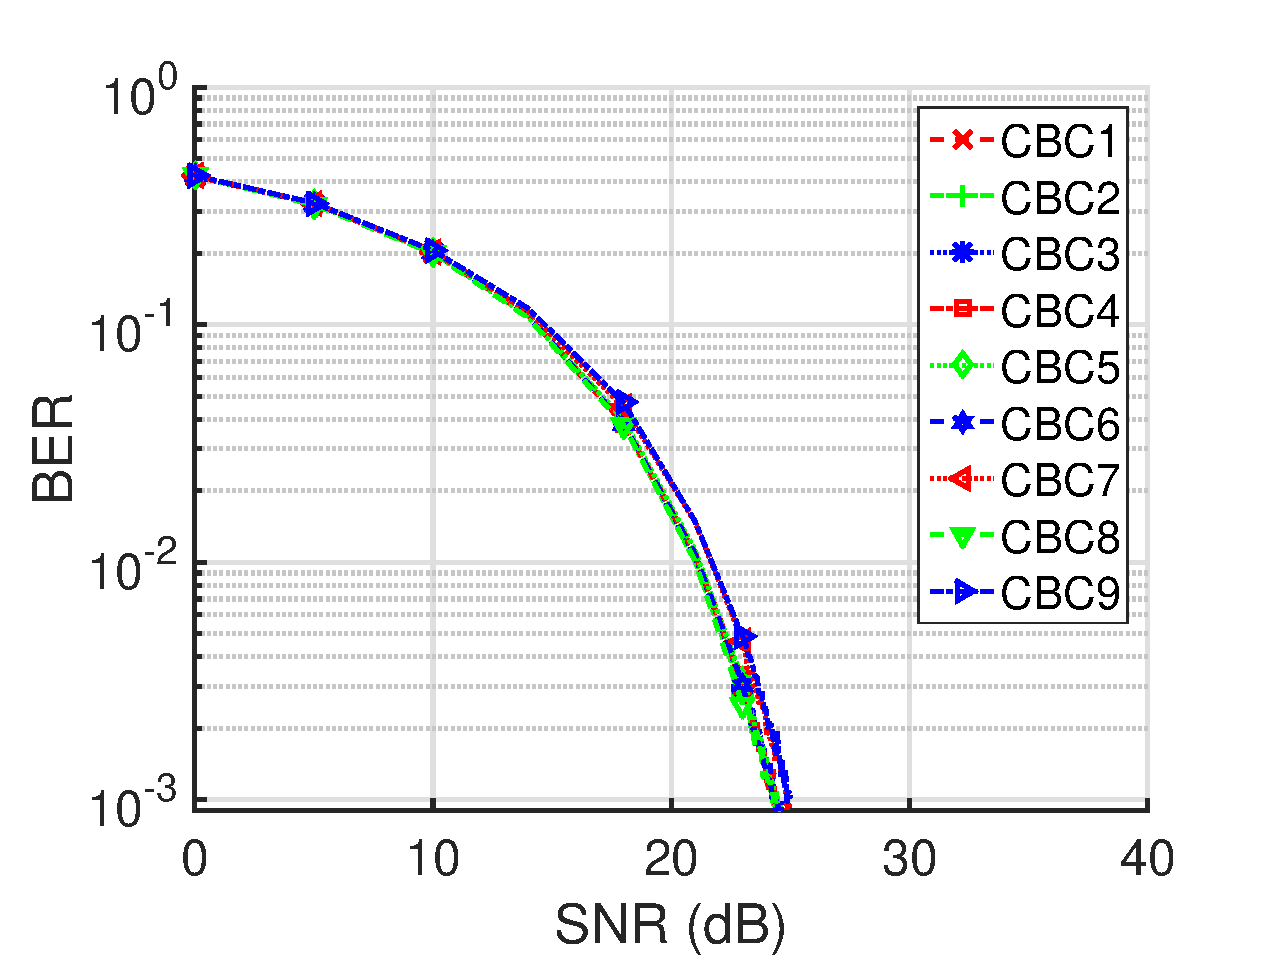
\includegraphics[trim={0.1in 0.0in 0.6in 0.3in}, clip=true, width=\textwidth]{M16_16-CSK_BERvsSNR.eps}
			\caption{16-CSK}
			\label{fig16SNR}
		\end{subfigure}
	\caption{BER vs SNR for linear model}
	\label{figBERvsSNR}
\end{figure}
\end{landscape}
\clearpage% Flush page
}

\figurename{ }\ref{figRcvSym} shows received symbols for CBC$_{2}$, whose constellation points are the most spread out, under the linear model. As expected, noise is spread normally along x and y dimensions forming a circular envelop around all constellation points. For $M$ = 8 and $M$ = 16, empty non-interfering regions devoid of received symbols can be seen in the figures. This indicates that these constellations could be better packed by defining additional points in the non-interfering regions. The constellations can then be further optimized to achieve better spectral efficiency. Note that in \figurename{ }\ref{figRcvSym} (\subref{fig4RcvSym}),
(\subref{fig8RcvSym}) and (\subref{fig16RcvSym}), some of the received
symbols are located outside the color gamut (triangle IJK
as outlined in \figurename{ }\ref{figConst}) formed by the sources for
i, j and k bands. This would appear to violate the relationships on the CIE-CS model between coordinates of SPDs of individual sources and that of the resultant SPD formed by mixing the fluxes in different ratios. However, at the receiver, the
received signals are influenced by noise (bipolar, zero-mean Gaussian)
resulting in bipolar received values. Received signals with negative values when mapped back to the CIE-CS, can cause received `noisy' symbols to lie outside of the gamut.

Since the transmitted radiant fluxes are always non-negative, it is possible to clip the receiver output prior to estimating the transmitted
radiant flux.  When negative receiver output is clipped at zero, estimated
symbols are illustrated in
\figurename{ }\ref{figRcvSym} (\subref{fig4RcvSymY0}),
(\subref{fig8RcvSymY0}) and (\subref{fig16RcvSymY0}). This
clipping shows that the mapping back to CIE-CS is sensical. It can also be seen that at target BER of $10^{-3}$, the clipping does not
introduce any significant change in performance when compared to that without clipping.

While this linear system model is instructive to study $M$-ary CSK modulation
and carry out a first order performance analysis, a practical CSK
system incorporating human eye's visual perception, is non-linear due to non-linearity of the CIE-CS. The ($x_{\text{p}}$, $y_{\text{p}}$) $\rightarrow  \text{P}_{n}$ block at the transmitter and its counterpart and $\hat{\text{P}}_{n}\rightarrow$ ($\hat{x}_{\text{p}}$, $\hat{y}_{\text{p}}$) at the receiver (red colored dashed
blocks in \figurename{ }\ref{figCSKBD}) introduce this non-linearity
which significantly alters the $M$-ary CSK performance for a practical
implementation. The effects of these practical constraints on a CSK
system are studied in next few sub-sections.

\afterpage{%
\clearpage
\begin{landscape}% Landscape page
\begin{figure}[t]
	\centering
		\begin{subfigure}{0.35\textwidth}
		\centering
			\includegraphics[trim={1.0in 0.0in 1.3in 0.1in}, clip=true, width=\textwidth]{M04_4-CSK_CBC2_ReceivedSymbols2.eps}
			\caption{4-CSK}
			\label{fig4RcvSym}
		\end{subfigure}
		%\hfill
		\begin{subfigure}{0.35\textwidth}
		\centering
			\includegraphics[trim={1.0in 0.0in 1.3in 0.1in}, clip=true, width=\textwidth]{M08_8-CSK_CBC2_ReceivedSymbols2.eps}
			\caption{8-CSK}
			\label{fig8RcvSym}
		\end{subfigure}
		%\hfill
		\begin{subfigure}{0.35\textwidth}
		\centering
			\includegraphics[trim={1.0in 0.0in 1.3in 0.1in}, clip=true, width=\textwidth]{M16_16-CSK_CBC2_ReceivedSymbols3.eps}
			\caption{16-CSK}
			\label{fig16RcvSym}
		\end{subfigure}
		\vfill
		%%%%%%%%% Y0 %%%%%%%%%
		\begin{subfigure}{0.35\textwidth}
		\centering
			\includegraphics[trim={1.0in 0.0in 1.3in 0.1in}, clip=true, width=\textwidth]{M04_4-CSK_CBC2_ReceivedSymbols2_Y0.eps}
			\caption{4-CSK}
			\label{fig4RcvSymY0}
		\end{subfigure}
		%\hfill
		\begin{subfigure}{0.35\textwidth}
		\centering
			\includegraphics[trim={1.0in 0.0in 1.3in 0.1in}, clip=true, width=\textwidth]{M08_8-CSK_CBC2_ReceivedSymbols2_Y0.eps}
			\caption{8-CSK}
			\label{fig8RcvSymY0}
		\end{subfigure}
		%\hfill
		\begin{subfigure}{0.35\textwidth}
		\centering
			\includegraphics[trim={1.0in 0.0in 1.3in 0.1in}, clip=true, width=\textwidth]{M16_16-CSK_CBC2_ReceivedSymbols3_Y0.eps}
			\caption{16-CSK}
			\label{fig16RcvSymY0}
		\end{subfigure}
	\caption{Received symbols for CBC$_{2}$. (a),(b),(c): Receiver output not clipped. (d),(e),(f): Negative values of receiver output clipped at zero.}
	\label{figRcvSym}
\end{figure}
%\caption{Received symbols for CBC$_{2}$.  Receiver output not clipped. (\subref{fig4RcvSym}),(\subref{fig8RcvSym}),(\subref{fig16RcvSym}): (\subref{fig4RcvSymY0}),(\subref{fig8RcvSymY0}),(\subref{fig16RcvSymY0} : Negative values of receiver output clipped at zero.}
\end{landscape}
\clearpage% Flush page
}
\clearpage
%%%%%%%%%%%%%%%%%%%  Non-linear Model  %%%%%%%%%%%%%%%%%%%%%
\subsection{Non-Linear System Model}
\label{subsec:cskNonlinear}
To understand the source of non-linearity in the CSK system, let's take a look at the CIE-CS which empirically models the human eye's visual perception of color for a stimulating SPD. Let $S_{n}(\lambda)$ be the SPDs of the transmit LEDs and P$_{n}$ be the radiant flux associated with band $n$. Thus the aggregate transmitted SPD is given by Eq.\eqref{eqWLDA}.

\begin{figure}[!b]
	\centering
		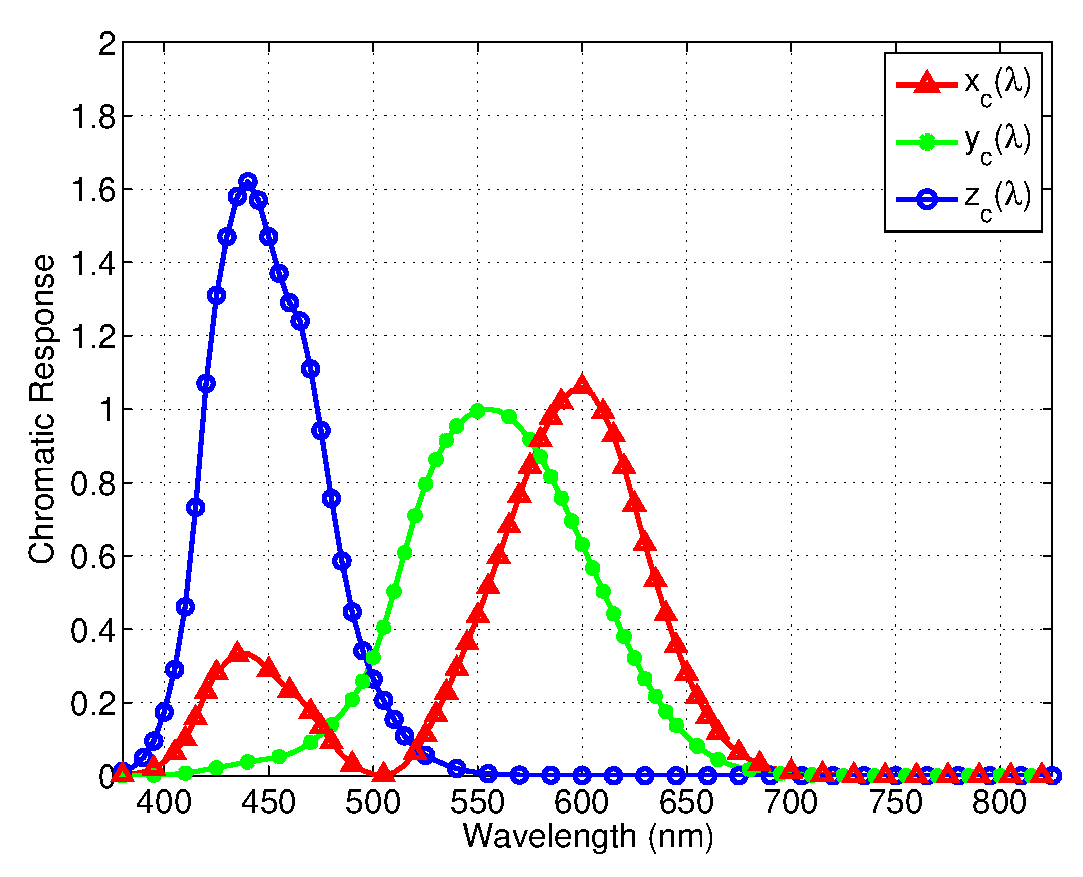
\includegraphics[trim={0.05in 0.05in 0.05in 0.05in}, clip=true, width=3.0in]{CIE1931CMF.eps}
	\caption{CIE 1931 XYZ color matching functions.}
	\label{figCIEXYZ}
\end{figure}

\begin{equation}
	W(\lambda) = \sum\limits_{n\text{ }\in\text{ \{i, j, k\}}}\text{P}_{n}S_{n}(\lambda)
	\label{eqWLDA}
\end{equation}

CIE-CS specification outlines three color matching functions - $x_{c}(\lambda)$, $y_{c}(\lambda)$ and $z_{c}(\lambda)$ as illustrated in \figurename{ }\ref{figCIEXYZ}. The tristimulus values for the three primary sources as defined in the CIE-CS are given by Eq.\eqref{eqTXYZ} and the chromaticity coordinates ($x_{\text{p}}$, $y_{\text{p}}$) of the resultant SPD $W(\lambda)$ are given by Eq.\eqref{eqWXY}. From Eqs.(\ref{eqWLDA}-\ref{eqWXY}) it can also be inferred that the relationship between P$_{n}$ and ($x_{\text{p}}$, $y_{\text{p}}$) is non-linear.

\begin{equation}
	\begin{aligned}
		X_{W} &= \int\limits_{\lambda\text{ = 380 nm}}^{\lambda\text{ = 780 nm}}W(\lambda)x_{c}(\lambda)d\lambda\\
		Y_{W} &= \int\limits_{\lambda\text{ = 380 nm}}^{\lambda\text{ = 780 nm}}W(\lambda)y_{c}(\lambda)d\lambda\\
		Z_{W} &= \int\limits_{\lambda\text{ = 380 nm}}^{\lambda\text{ = 780 nm}}W(\lambda)z_{c}(\lambda)d\lambda
	\end{aligned}
	\label{eqTXYZ}
\end{equation}

\begin{equation}
	x_{\text{p}} = \frac{X_{W}}{X_{W}+Y_{W}+Z_{W}}; \text{  } y_{\text{p}} = \frac{Y_{W}}{X_{W}+Y_{W}+Z_{W}} % \text{  } adds space.
	\label{eqWXY}
\end{equation}

As outlined in prior sections, $M$-ary CSK modulation transmits information by varying the chromaticity coordinates of transmit SPD. In a practical implementation, a table of unique transformation ratios P$_{\text{i}}$:P$_{\text{j}}$:P$_{\text{k}}$ $\rightarrow$ $(x_{\text{p}},y_{\text{p}})$ can be pre-computed for each of the $M$ constellation points. Referring back to \figurename{ }\ref{figCSKBD}, at the transmitter the data is color coded to obtain ($x_{\text{p}}$, $y_{\text{p}}$) coordinate to transmit. Given this coordinate, corresponding flux ratios P$_{\text{i}}$:P$_{\text{j}}$:P$_{\text{k}}$ can be looked up from the pre-computed table. The target illumination requirements provide the total radiant flux to output from the transmitting sources. With the flux ratio and the total radiant flux information, individual P$_{n}$ for each band $n$ can now be computed from Eq.\eqref{eqWLDA}. This transformation now forms the ($x_{\text{p}}$, $y_{\text{p}}$) $\rightarrow  \text{P}_{n}$ block in the transmitter signaling chain. These transmitted flux are sensed by the receivers in presence of AWGN. The receivers generate an electrical output which is then used to compute an estimate of transmitted radiant fluxes $\hat{\text{P}}_{n}$. Eqs.(\ref{eqWLDA}-\ref{eqWXY}), which now constitute the $\hat{\text{P}}_{n}\rightarrow$ ($\hat{x}_{\text{p}}$, $\hat{y}_{\text{p}}$) block in the receive signal chain, can then be used to estimate the transmitted coordinate ($\hat{x}_{\text{p}}$, $\hat{y}_{\text{p}}$). Thus, the AWGN added to the received signal undergoes a non-linear transformation during $\hat{\text{P}}_{n}\rightarrow$ ($\hat{x}_{\text{p}}$, $\hat{y}_{\text{p}}$) process which skews the noise in the chromaticity plane of the CIE-CS. This causes additional performance penalties in a practical CSK system.

\afterpage{%
\clearpage
\begin{landscape}% Landscape page
\begin{figure}[t]
	\centering
		\begin{subfigure}{0.49\textwidth}
		\centering
			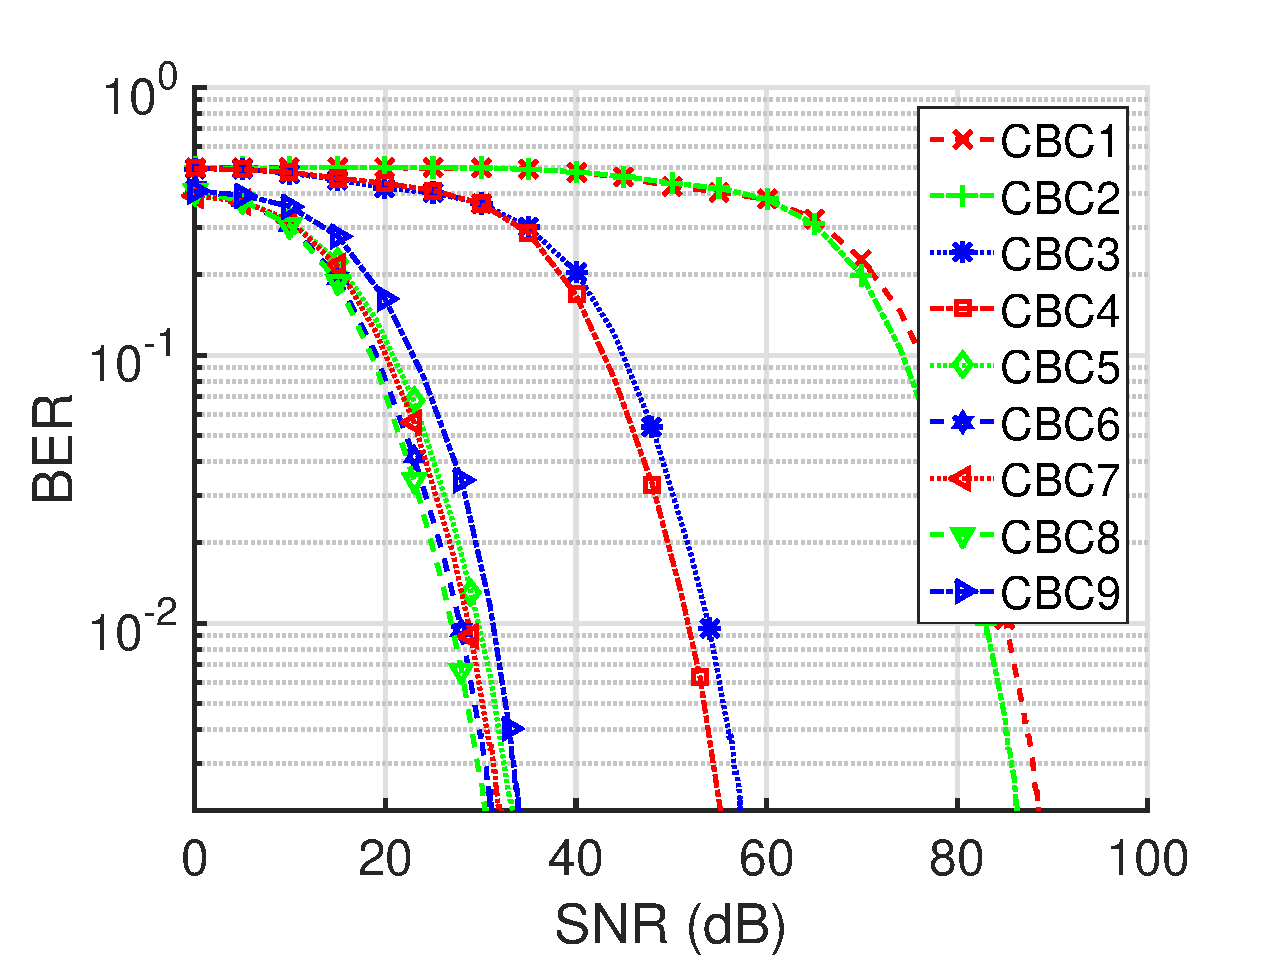
\includegraphics[trim={0.1in 0.0in 0.5in 0.3in}, clip=true, width=\textwidth]{M04_4-CSK_BERvsSNR_NL.eps}
			\caption{4-CSK}
			\label{fig4SNR_NL}
		\end{subfigure}
		%\hfill
		\begin{subfigure}{0.49\textwidth}
		\centering
			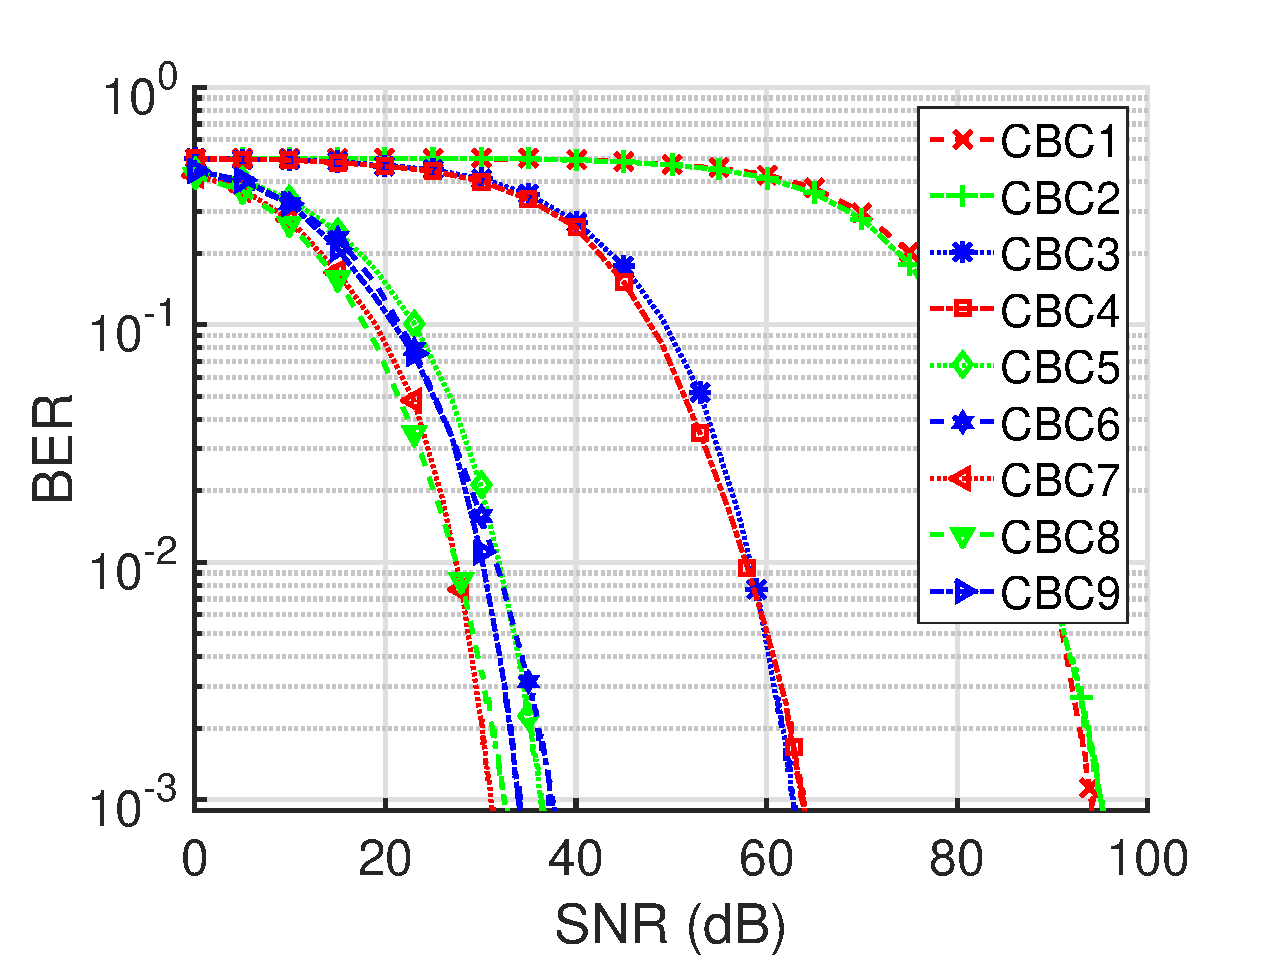
\includegraphics[trim={0.1in 0.0in 0.5in 0.3in}, clip=true, width=\textwidth]{M08_8-CSK_BERvsSNR_NL.eps}
			\caption{8-CSK}
			\label{fig8SNR_NL}
		\end{subfigure}
		%\vfill
		\begin{subfigure}{0.49\textwidth}
		\centering
			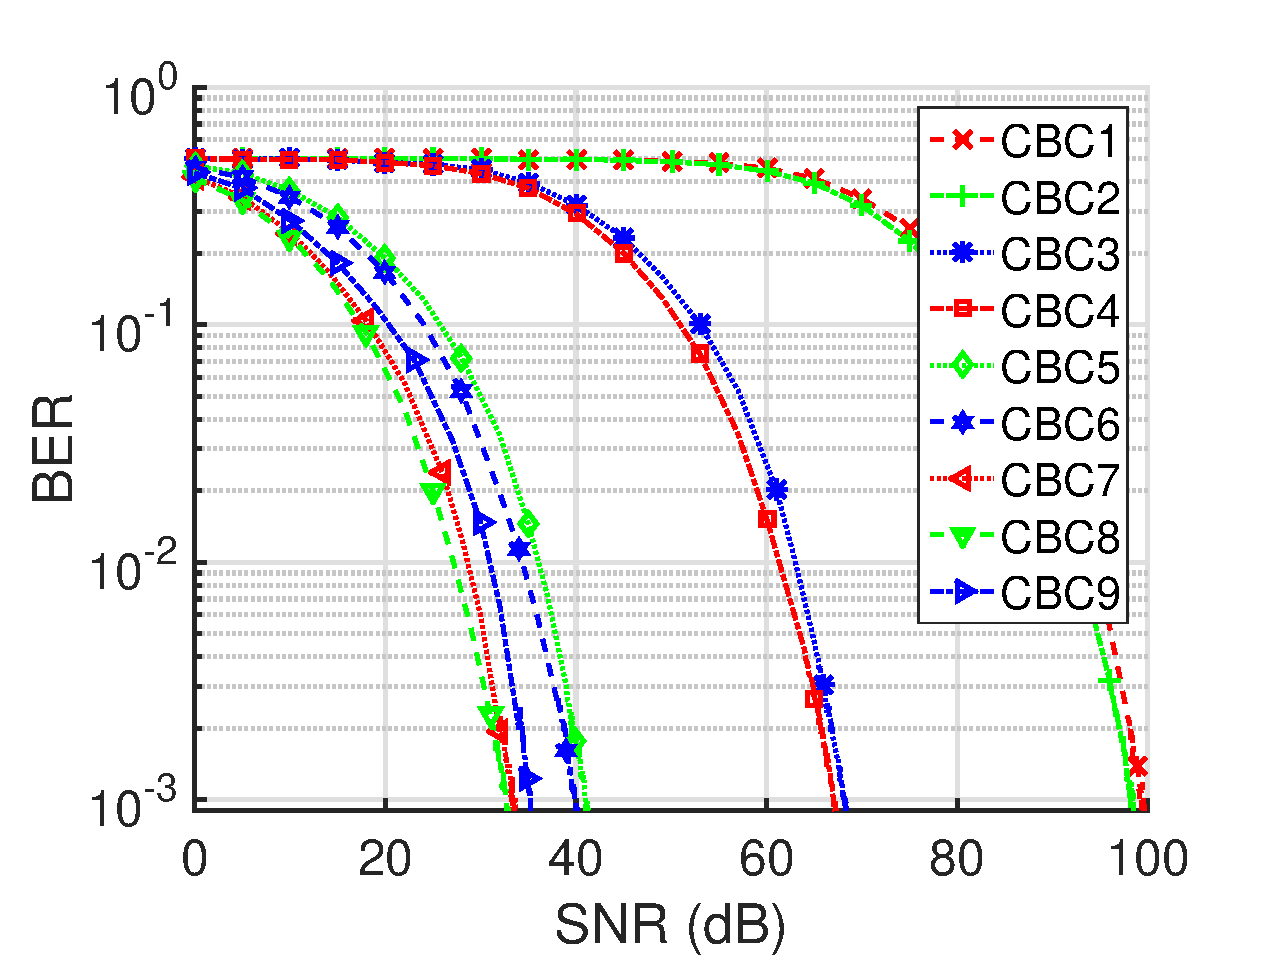
\includegraphics[trim={0.1in 0.0in 0.5in 0.3in}, clip=true, width=\textwidth]{M16_16-CSK_BERvsSNR_NL.eps}
			\caption{16-CSK}
			\label{fig16SNR_NL}
		\end{subfigure}
	\caption{BER vs SNR for all CBC}
	\label{figBERvsSNR_NL}
\end{figure}
\end{landscape}
\clearpage% Flush page
}

\figurename{ }\ref{figBERvsSNR_NL} shows performance of all the CBCs under this non-linear model. These curves are obtained by monte-carlo simulations similar to those performed for the linear model after substituting the P$_{n}$ $\rightarrow$ ($x_{\text{p}}$, $y_{\text{p}}$) and $\hat{\text{P}}_{n}\rightarrow$ ($\hat{x}_{\text{p}}$, $\hat{y}_{\text{p}}$) blocks with the non-linear system model transformations. It can be observed that CBC$_{7}$ and CBC$_{8}$ perform relatively similar and are the best while CBC$_{1}$ performs the worst. Additionally, it is observed that CBC$_{1}$-CBC$_{4}$ perform significantly worse as compared to the rest. For CBC$_{1}$-CBC$_{4}$, the amount of radiant flux emitted by band i is 3-4 orders of magnitude greater than band j and 1-2 orders of magnitude greater than band k. Thus the $\hat{\text{P}}_{n}\rightarrow$ ($\hat{x}_{\text{p}}$, $\hat{y}_{\text{p}}$) conversion at the receiver is extremely sensitive to noise along the j and k bands as compared to that along the i band. This introduces significant errors in decoding received symbols.

\afterpage{%
\clearpage
\begin{landscape}% Landscape page
\begin{figure}[t]
	\centering
		%%%%%%%%% CBC1 %%%%%
		\begin{subfigure}{0.35\textwidth}
		\centering
			\includegraphics[trim={1.0in 0.0in 1.3in 0.1in}, clip=true, width=\textwidth]{M04_4-CSK_CBC1_ReceivedSymbols9_NL.eps}
			\caption{CBC$_{1}$: 4-CSK}
			\label{fig4RcvSym_NL1}
		\end{subfigure}
		%%\hfill
		\begin{subfigure}{0.35\textwidth}
		\centering
			\includegraphics[trim={1.0in 0.0in 1.3in 0.1in}, clip=true, width=\textwidth]{M08_8-CSK_CBC1_ReceivedSymbols10_NL.eps}
			\caption{CBC$_{1}$: 8-CSK}
			\label{fig8RcvSym_NL1}
		\end{subfigure}
		%\hfill
		\begin{subfigure}{0.35\textwidth}
		\centering
			\includegraphics[trim={1.0in 0.0in 1.3in 0.1in}, clip=true, width=\textwidth]{M16_16-CSK_CBC1_ReceivedSymbols10_NL.eps}
			\caption{CBC$_{1}$: 16-CSK}
			\label{fig16RcvSym_NL1}
		\end{subfigure}
		%\vfill
		%%%%%%%%% CBC8 %%%%%
		\begin{subfigure}{0.35\textwidth}
		\centering
			\includegraphics[trim={1.0in 0.0in 1.3in 0.1in}, clip=true, width=\textwidth]{M04_4-CSK_CBC8_ReceivedSymbols4_NL.eps}
			\caption{CBC$_{8}$: 4-CSK}
			\label{fig4RcvSym_NL8}
		\end{subfigure}
		%\hfill
		\begin{subfigure}{0.35\textwidth}
		\centering
			\includegraphics[trim={1.0in 0.0in 1.3in 0.1in}, clip=true, width=\textwidth]{M08_8-CSK_CBC8_ReceivedSymbols4_NL.eps}
			\caption{CBC$_{8}$: 8-CSK}
			\label{fig8RcvSym_NL8}
		\end{subfigure}
		%\hfill
		\begin{subfigure}{0.35\textwidth}
		\centering
			\includegraphics[trim={1.0in 0.0in 1.3in 0.1in}, clip=true, width=\textwidth]{M16_16-CSK_CBC8_ReceivedSymbols4_NL.eps}
			\caption{CBC$_{8}$: 16-CSK}
			\label{fig16RcvSym_NL8}
		\end{subfigure}
	\caption{Received symbols for non-linear model when receiver output is not clipped. Some received symbols are located outside the color gamut. Note that noise when transformed to chromaticity plane is no longer AWGN.}
	\label{figRcvSym_NL}
\end{figure}
\end{landscape}
\clearpage% Flush page
}

\afterpage{%
\clearpage
\begin{landscape}% Landscape page
\begin{figure}[t]
	\centering
	%%%%%%%%% CBC1 Y0 %%%%%
		\begin{subfigure}{0.35\textwidth}
		\centering
			\includegraphics[trim={1.0in 0.0in 1.3in 0.1in}, clip=true, width=\textwidth]{M04_4-CSK_CBC1_ReceivedSymbols9_NL_Y0.eps}
			\caption{CBC$_{1}$: 4-CSK}
			\label{fig4RcvSym_NL1_Y0}
		\end{subfigure}
		%\hfill
		\begin{subfigure}{0.35\textwidth}
		\centering
			\includegraphics[trim={1.0in 0.0in 1.3in 0.1in}, clip=true, width=\textwidth]{M08_8-CSK_CBC1_ReceivedSymbols10_NL_Y0.eps}
			\caption{CBC$_{1}$: 8-CSK}
			\label{fig8RcvSym_NL1_Y0}
		\end{subfigure}
		%\hfill
		\begin{subfigure}{0.35\textwidth}
		\centering
			\includegraphics[trim={1.0in 0.0in 1.3in 0.1in}, clip=true, width=\textwidth]{M16_16-CSK_CBC1_ReceivedSymbols10_NL_Y0.eps}
			\caption{CBC$_{1}$: 16-CSK}
			\label{fig16RcvSym_NL1_Y0}
		\end{subfigure}
		%\vfill
		%%%%%%%%% CBC8 Y0 %%%%%
		\begin{subfigure}{0.35\textwidth}
		\centering
			\includegraphics[trim={1.0in 0.0in 1.3in 0.1in}, clip=true, width=\textwidth]{M04_4-CSK_CBC8_ReceivedSymbols4_NL_Y0.eps}
			\caption{CBC$_{8}$: 4-CSK}
			\label{fig4RcvSym_NL8_Y0}
		\end{subfigure}
		%\hfill
		\begin{subfigure}{0.35\textwidth}
		\centering
			\includegraphics[trim={1.0in 0.0in 1.3in 0.1in}, clip=true, width=\textwidth]{M08_8-CSK_CBC8_ReceivedSymbols4_NL_Y0.eps}
			\caption{CBC$_{8}$: 8-CSK}
			\label{fig8RcvSym_NL8_Y0}
		\end{subfigure}
		%\hfill
		\begin{subfigure}{0.35\textwidth}
		\centering
			\includegraphics[trim={1.0in 0.0in 1.3in 0.1in}, clip=true, width=\textwidth]{M16_16-CSK_CBC8_ReceivedSymbols4_NL_Y0.eps}
			\caption{CBC$_{8}$: 16-CSK}
			\label{fig16RcvSym_NL8_Y0}
		\end{subfigure}
	\caption{Received symbols for non-linear model when negative values of receiver output are clipped at zero. All received symbols now are located inside the color gamut. Note that noise when transformed to chromaticity plane is no longer AWGN.}
	\label{figRcvSym_NL_Y0}
\end{figure}
\end{landscape}
\clearpage% Flush page
}

\figurename{ }\ref{figRcvSym_NL} and \figurename{ }\ref{figRcvSym_NL_Y0} show received symbols for CBC$_{1}$ and CBC$_{8}$ under the non-linear model. Noise skew about the estimated coordinates can be observed in both figures. This noise skew is more prominent for CBC$_{1}$ where the signal power distribution along all bands is imbalanced. In contrast for CBC$_{8}$, signal power is more uniformly spread across all bands. For \figurename{ }\ref{figRcvSym_NL}, the negative receiver output is not clipped at zero. As mentioned earlier, in presence of noise (zero mean and Gaussian), some receiver output values can be negative and thus such received symbols are located outside the color gamut when transformed to CIE-CS space. The effect of clipping negative receiver output at zero can be seen in \figurename{ }\ref{figRcvSym_NL_Y0} where all received symbols now are located inside the color gamut. It can be seen that performance of both receiver signal processing techniques is similar, as such no one outperforms the other. It can be seen that AWGN introduced on $\hat{\text{P}}_{n}$ gets skewed radially towards band k due to non-linearity in $\hat{\text{P}}_{n}\rightarrow$ ($\hat{x}_{\text{p}}$, $\hat{y}_{\text{p}}$) transformation and is no longer AWGN along the CIE-CS chromaticity plane. This generates an interesting outcome in that for CBC$_{8}$, about 30 dB of SNR is needed to achieve target $10^{-3}$ BER for all of $M$ = 4, 8 and 16 CSK. This happens because with increase in order $M$, the additional constellation points as defined in the standard happen to occupy non-interfering regions of the chromaticity plane thus increasing spectral efficiency without incurring any SNR penalty up to a point. The non-linearity of the CIE-CS introduces performance penalties of at least 15 dB, 10 dB and 5 dB for $M$ = 4, 8 and 16 CSK respectively over the linear system model. 

%%%%%%%%%%%%%%%%%%%%%  Illumination  %%%%%%%%%%%%%%%%%%%%%%%
\subsection{CSK: Performance under illumination constraints}
\label{subsec:cskIllumination}

%%%%%%%%%%%%  Luminous Signal to Noise Ratio  %%%%%%%%%%%%%%
%\subsection{Luminous-signal-to-noise ratio}\label{ssLSNR}
In an indoor optical wireless system using lighting devices for wireless downlink access the luminaires need to simultaneously service illumination and optical wireless broadcast missions. Under this model, different colored PHY (example: different CBC$_{v}$) irradiate different amounts of radiant flux to achieve the same illumination intensity level. Thus, it is unfair to use SNR as a metric to compare performance of modulation schemes at same BER target using different colored PHY without first normalizing for illumination targets. Thus, in this section we introduce LSNR as a metric that takes into account the differences in radiant flux emitted by different PHY to achieve the same illumination intensity level. It should be noted that the LSNR metric is not specific to CSK, but instead can be used more generally to compare performance of any two optical modulation schemes that are operated at the same optical intensity levels.

\afterpage{%
\clearpage
\begin{landscape}% Landscape page
\begin{figure}[b]
	\centering
		\begin{subfigure}{0.49\textwidth}
		\centering
			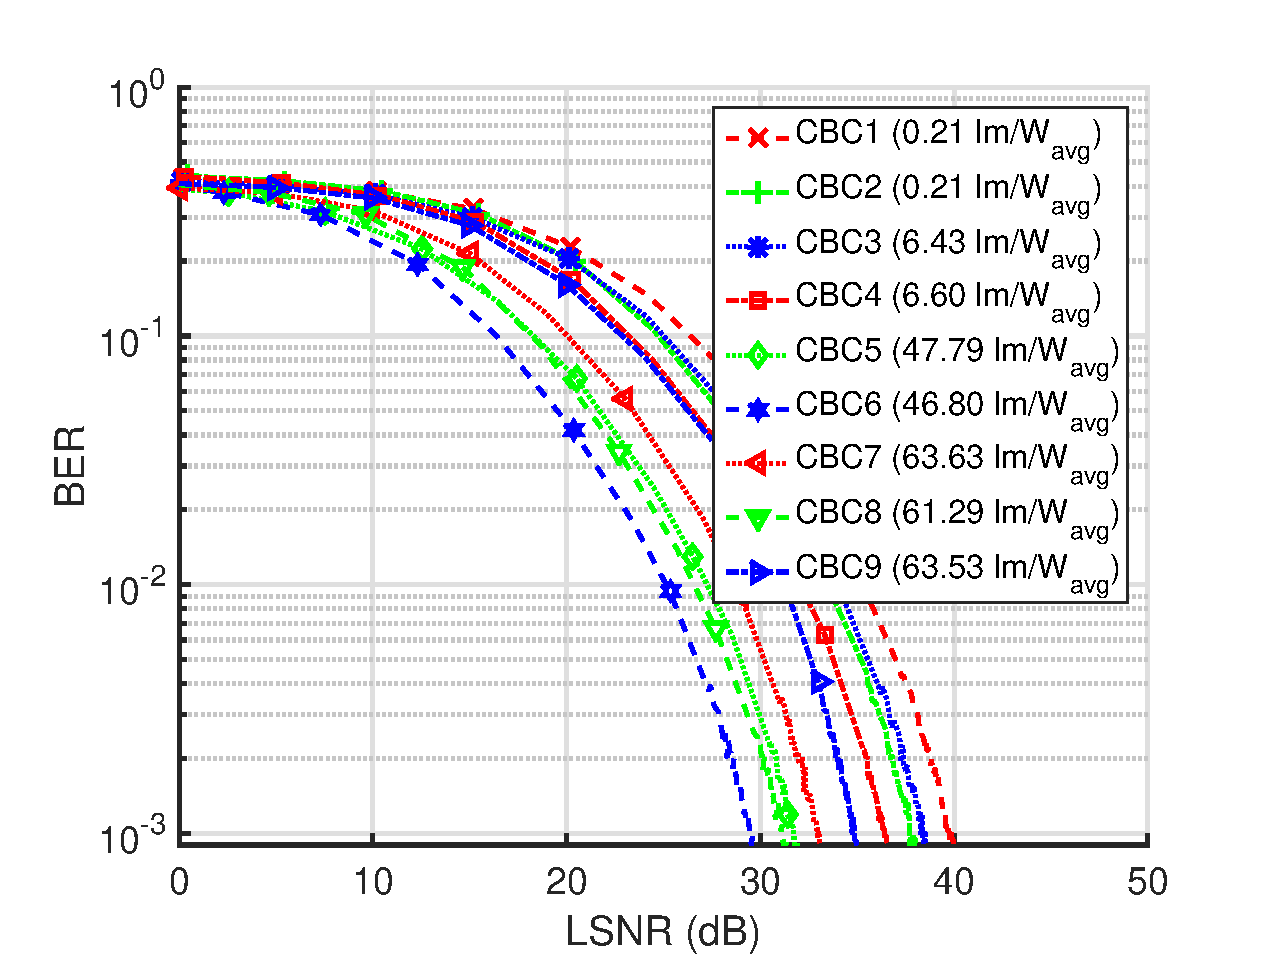
\includegraphics[trim={0.1in 0.0in 0.5in 0.1in}, clip=true, width=\textwidth]{M04_4-CSK_BERvsLSNR_NL.eps}
			\caption{4-CSK}
			\label{fig4LSNR}
		\end{subfigure}
		%\hfill
		\begin{subfigure}{0.49\textwidth}
		\centering
			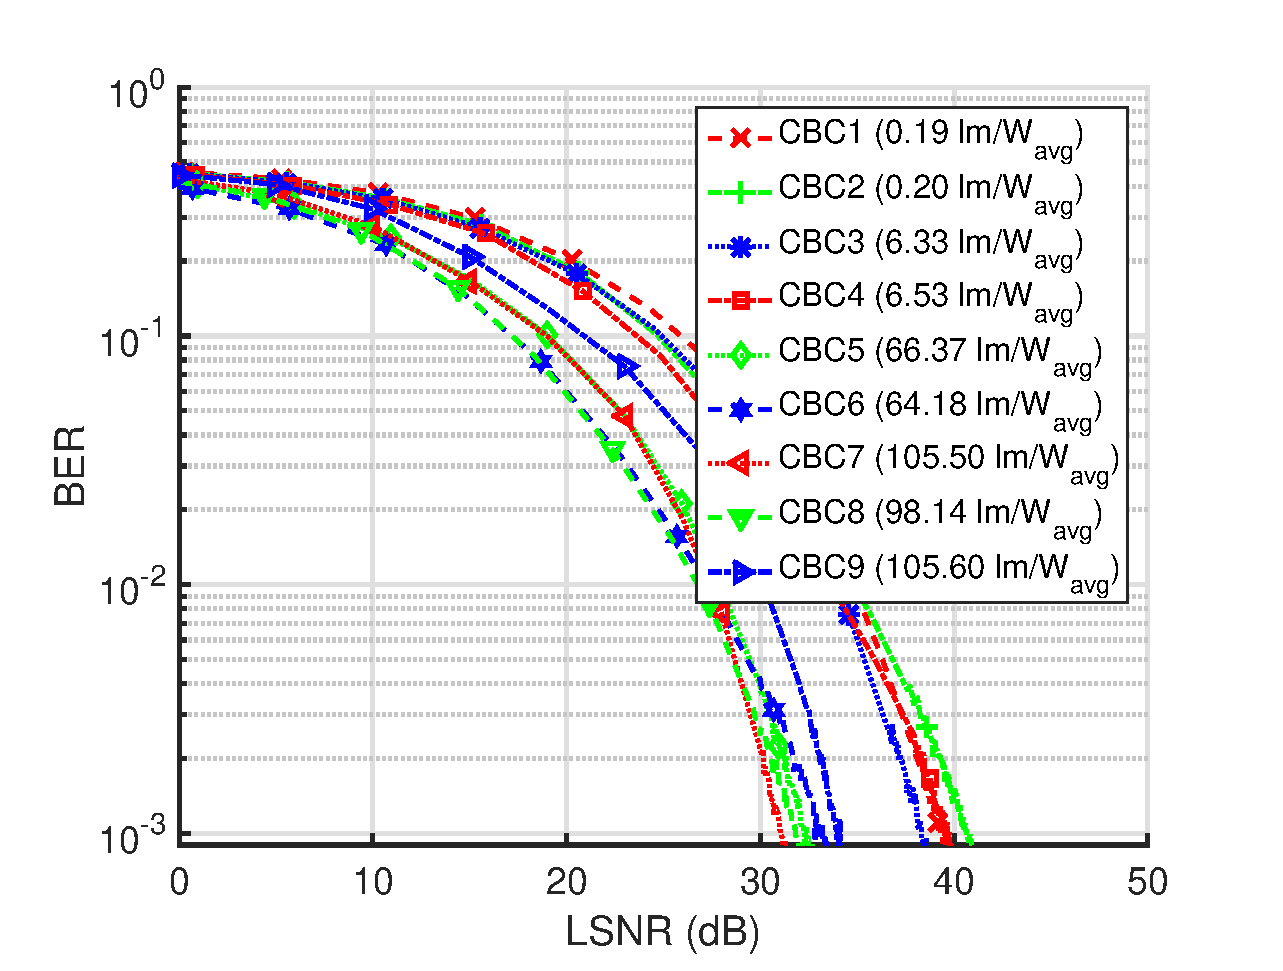
\includegraphics[trim={0.1in 0.0in 0.5in 0.1in}, clip=true, width=\textwidth]{M08_8-CSK_BERvsLSNR_NL.eps}
			\caption{8-CSK}
			\label{fig8LSNR}
		\end{subfigure}
		%\vfill
		\begin{subfigure}{0.49\textwidth}
		\centering
			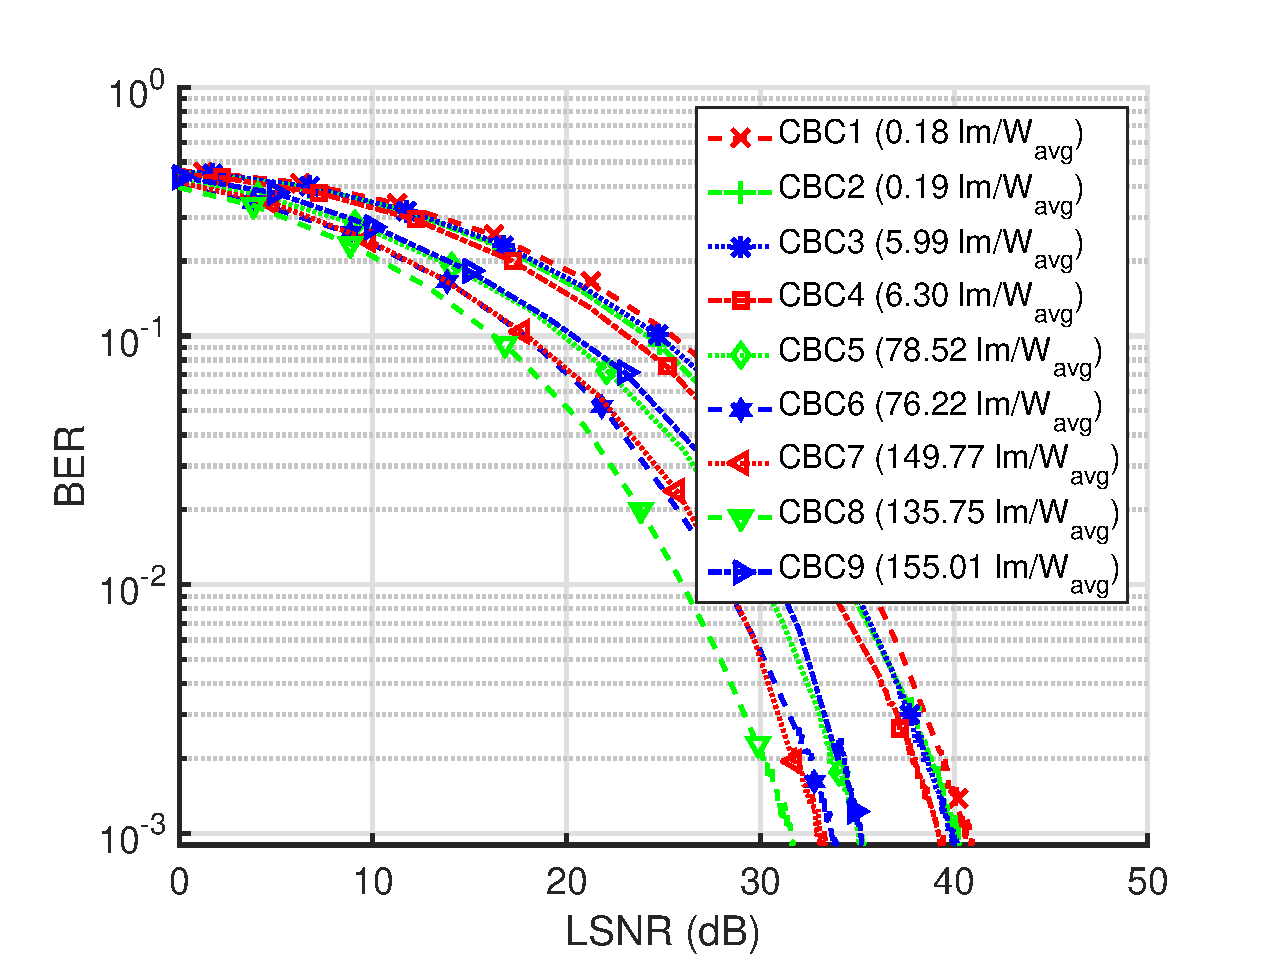
\includegraphics[trim={0.1in 0.0in 0.5in 0.1in}, clip=true, width=\textwidth]{M16_16-CSK_BERvsLSNR_NL.eps}
			\caption{16-CSK}
			\label{fig16LSNR}
		\end{subfigure}
	\caption{BER vs LSNR for all CBC}
	\label{figBERvsLSNR}
\end{figure}
\end{landscape}
\clearpage% Flush page
}

Consider optical modulation scheme(s) which can be implemented with two different constellations C$_{\text{a}}$ or C$_{\text{b}}$. The fluxes emitted by the two constellations are scaled to achieve a target illumination intensity level. Let both constellations on average emit I lumens of luminous flux. Let the luminous efficacy for the two constellations be specified by $\eta_{\text{a}}$ and $\eta_{\text{b}}$ in lumens-per-watt respectively. Then the corresponding average radiant flux emitted by the two constellations is given by W$_{\text{a}}$ = I/$\eta_{\text{a}}$ and W$_{\text{b}}$  = I/$\eta_{\text{b}}$ watts respectively. Let us define a luminous ratio L$_{\text{ab}}\triangleq$ ($\eta_{\text{a}}/\eta_{\text{b}}$) $\equiv$ (W$_{\text{b}}$/W$_{\text{a}}$). Thus, for every 1 Watt of radiant flux emitted by C$_{\text{a}}$, C$_{\text{b}}$ must emit L$_{\text{ab}}$ Watt of radiant flux to achieve the same illumination intensity level. Under the model where the luminaires service illumination along with communication, it is fair to compare the performance of the two schemes at these relative radiant flux levels instead of at the absolute radiant flux levels. Thus we define the LSNR metric in Eq.\eqref{eqLSNR} as a means to compare performance of C$_{\text{b}}$ versus that of C$_{\text{a}}$ at same illumination levels. 

\begin{equation}
	% ^{ } is used with \vm{X} to help align subscript 'b' for both \vm{X} below.
	\text{LSNR}_{\text{ab}} \triangleq \frac{\text{L}^{2}_{\text{ab}}\text{Tr}\{\vm{H}\vm{X}^{ }_{\text{b}}\vm{X}^{*}_{\text{b}}\vm{H}^{*}\}}{\sigma^{2}_{n}} 
	\label{eqLSNR}
\end{equation}
where \vm{X}$_{\text{b}}$ is the average radiant flux emitted by C$_{\text{b}}$. Thus, after computing BER vs SNR for the scheme employing C$_{\text{a}}$, BER vs LSNR can be computed for scheme employing C$_{\text{b}}$ to compare its performance relative to that employing C$_{\text{a}}$ at the same illumination levels.

%%%%%%%%%%%%%%%%%%%%%  Illumination  %%%%%%%%%%%%%%%%%%%%%%%
%\subsection{Performance under illumination constraints}\label{ssCSKLSNR}

\figurename{ }\ref{figBERvsLSNR} shows performance of the 9 CBCs under the non-linear model when normalized for illumination constraints. The efficacies of all CBC for different $M$ are specified in the legends. These values are used to normalize the performance of $M$-ary CSK for all CBC using CBC with highest efficacy as the reference for LSNR calculation. CBC$_{7}$, CBC$_{9}$ and CBC$_{9}$ are used as reference CBCs for $M$ = 4, 8 and 16 CSK respectively. The effect of this is to shift all curves (except the reference) from \figurename{ }\ref{figBERvsSNR_NL} towards left along the LSNR-axis depending on the L$_{\text{ab}}$ values in Eq.\eqref{eqLSNR}. It can be observed that given a target illumination intensity level and for target 10$^{-3}$ BER, CBC$_{6}$ performs the best for 4-CSK, CBC$_{7}$ and CBC$_{8}$ perform similar and better than others for 8-CSK and CBC$_{8}$ performs the best for 16-CSK. For CBC$_{1}$-CBC$_{4}$, due to their low luminous efficacy, one can use a much larger radiant flux to achieve target illumination levels and thus significantly improve their communication performance. However, this is achieved at the cost of poor energy efficiency. In contrast, CBC$_{7}$ and CBC$_{9}$ have relatively high luminous efficacy. This implies that these CBCs are restricted to emit a relatively lower radiant flux (and thus low signal powers) to achieve target illumination level thus affecting their communication performance. These results also highlight the necessary tradeoff between goals of energy efficient lighting and good communication performance; thus making a case for an optimization between the two divergent goals.
